\chapter{Introducción} % Main chapter title

\label{Chapter1} % For referencing the chapter elsewhere, use \ref{Chapter1} 
\label{IntroGeneral}


%----------------------------------------------------------------------------------------

%\section{Introducción}

%----------------------------------------------------------------------------------------
\section{Motivación y Objetivos}
\label{sec:MotivacionyObjetivos}

La generación de residuos es uno de los principales problemas ambientales, económicos y de salud del planeta según el programa de Las Naciones Unidas para el Medio Ambiente\citep{GWMO2024}, sobre todo en el último siglo con una expansión económica basada en el consumo.

Se estima que a nivel mundial se producen alrededor de 4000 millones de toneladas de residuos al año y en nuestro país alrededor de 20 millones. Las grandes ciudades invierten una cuantiosa cantidad de dinero en recolección y disposición de residuos sólidos urbanos mientras que ciudades más pequeñas tienen serias dificultades para controlar los basurales a cielo abierto, convirtiendo a estos en focos de contaminación.
La principal sugerencia para mitigar esta problemática se encuentra definida en el concepto de la triple R, Reducir, Reciclar y Reusar.

La técnica de compostaje comprende el concepto de la triple R, siendo que su actividad permite reducir la cantidad de residuo orgánico mediante su reciclado, transformándolo en un mejorador de suelos para beneficio de las plantas.

Se considera que del 30 al 60\% del peso de una bolsa de basura generada en un hogar corresponde a material orgánico, residuos que mediante un proceso biológico controlado y monitoreado puede convertirse en abono orgánico.

Este proyecto consiste en desarrollar una solución de bajo costo que contribuya a monitorear los distintos parámetros que se deben tener en cuenta en el proceso de descomposición de los residuos orgánicos, para obtener como resultado un compost de buena calidad.

\section{Compost - Parámentros y su importancia}
\label{sec:CompostParámentros}

Determinados parámetros son importantes indicadores del proceso de descomposición de la materia orgánica. Un buen seguimiento garantiza que la transformación de la materia se desarrolle de manera eficiente y produzca un compost de alta calidad.
A continuación, se explican los parámetros más relevantes y la información útil que proporcionan \citep{ManualBuenasPracticas}:

 \begin{enumerate}
	\item Temperatura: la temperatura es importante para monitorear la actividad microbiana en el compost. Tal como se indica en la figura \ref{fig:curvatemp}, se observan tres fases en el proceso de descomposición aeróbica dentro de una pila de compost: fase mesófila inicial (Temperatura < 45°); fase termófila (Temperatura > 45°); y fase mesófila final, considerándose finalizado el proceso cuando se alcanza nuevamente la temperatura inicial.
    Cada especie de microorganismo tiene un intervalo de temperatura óptimo para su actividad: 15-40°C para los microorganismos mesófilos y 40-70°C para los termófilos \citep{FactoresCompost}. Es la actividad de estos microorganismos la generadora de calor.
    \item Humedad: la presencia de agua es indispensable para la descomposición de la materia orgánica. La humedad óptima para el crecimiento microbiano está entre 50-70\%; la actividad biologica decrece mucho cuando la humedad esta por debajo del 30\%; por encima del 70\% el agua desplaza el aire en los espacios libres existentes entre las particulas de materia orgánica reduciendo la transferencia de oxígeno y produciendo una anaerobiosis \citep{Compost}.
    \item pH: mediante el seguimiento del pH se puede obtener una medida indirecta del control de la aireación de la mezcla, ya que si en algún momento se crean condiciones anaeróbicas se liberan ácidos que provocan el descenso del pH. Al igual que con la temperatura, el pH presenta tres fases \citep{FactoresCompost}.
    \item Relación Carbono/Nitrógeno (C/N): esta relación determina el equilibrio entre materiales ricos en carbono (como hojas secas) y materiales ricos en nitrógeno (como restos de comida) \citep{FactoresCompost}.
    \item Textura y tamaño de las partículas: cuanto mayor sea la superficie expuesta al ataque microbiano por unidad de masa, más rápida sera la reacción. Pero es importante tener en cuenta que un tamaño más chico de partículas también reduce  el espacio libre entre ellas, desplazando o no dando lugar al oxígeno y compactando el compost \citep{ManualBuenasPracticas}.
    \item Contenido de nutrientes: las concentraciones de nutrientes como nitrógeno (N), fósforo (P) y potasio (K) determinan el valor y la calidad del compost como enmienda del suelo. Un compost bien balanceado debe tener una proporción adecuada de estos nutrientes para ser beneficiosos en la agricultura. \citep{Risti}
 \end{enumerate}
 

 \begin{figure}[H]
	\centering
	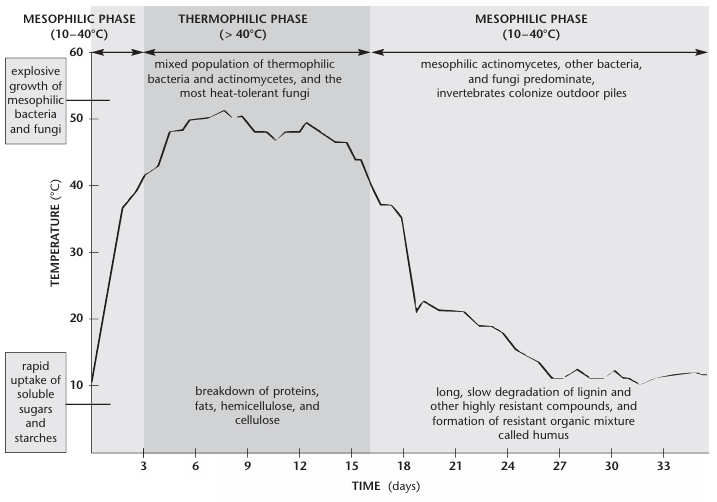
\includegraphics[scale=.7]{Figures/Compost Caracteristicas/Curva Temperatura.PNG}
	\caption{Curva característica de temperatura en una pila de compost \citep{curvaTemp}}
	\label{fig:curvatemp}
\end{figure}

\section{Estado Del Arte} % Main chapter title


\subsection{Estado del arte del compostaje en Argentina}
\label{sec:EstadoArteArgentina}

En Argentina, el compostaje se encuentra en una etapa inicial en cuanto a la adopción de tecnologías avanzadas para su monitoreo y control. La mayoría de las prácticas actuales son manuales y tradicionales y son muy pocos los organismos, entes o institutos que han adoptado alguna integración tecnológica (esto se debe principalmente por la falta de legislaciones en cuanto al tratamiento de residuos orgánicos).

\subsubsection{Desarrollos del INTA (Instituto Nacional de Tecnología Agropecuaria)}

El INTA trabajó hace unos años en una iniciativa donde se desarrollo un prototipo de sensores básicos para medir temperatura y humedad en compostajes rurales \footnote{Ver \url{https://intainforma.inta.gob.ar/desarrollan-sensor-para-optimizar-la-produccion-de-compost/}}. Sin embargo estos avances no han sidos implementados a nivel industrial o comercial hasta donde se ha podido investigar.

\subsubsection{Prácticas actuales}
A nivel industrial e individual, la mayoría de las maniobras relacionadas al compostaje se desarrollan de manera manual. Estas practicas incluyen:
\begin{itemize}
    \item Monitoreo de temperatura y humedad: la temperatura se miden empleando unos termómetros largos que se insertan en la pila de compost. Esta práctica se lleva a cabo varias veces por semana de manera de garantizar que el material en descomposición no alcance temperaturas críticas. Para la humedad se emplea el método del puño, que consiste en apretar una muestra de materia orgánica y observar si libera agua o se desmorona al soltarla.
    \item Volteo y aireación: en la mayoría de los casos, las pilas de compost son aireadas manualmente (por ejemplo mediante el uso de palas) o con maquinarias no especializadas (por ejemplo excavadoras).
\end{itemize}

Tal como se puede observar, las practicas actuales requieren la presencia de operarios en el lugar tanto sea para el monitoreo como para llevar a cabo acciones correctivas. Estas practicar aumentan la carga laboral y reducen la eficiencia del proceso; y exponen a un ambiente nocivo al operario en cuestión.

\subsection{Estado Del Arte del Compost a nivel global}
\label{sec:EstadoArteGlobal}

A nivel global las técnicas de compostaje han evolucionado significativamente y han surgido integraciones tecnológicas que permitieron optimizar el proceso, sobretodo en países con fuertes políticas de reciclaje y pioneros en innovación.
Se decidió detallar los casos de Estados Unidos y Japón para ejemplificar los avances a nivel global, ya que en otras partes del planeta y en países similares, los desarrollos se encuentran en fases similares.

\subsubsection{Estados Unidos}
En Estados Unidos existen soluciones privadas que integran IoT y automatizaciones para el monitoreo y procesamiento del compost. Dentro de ellas se destacan empresas como EcoRich \citep{ECORICH}

También destacan proyectos comunitarios, como el programa \textit{Zero Waste} \citep{ZeroWaste}, \textit{Farm Philly} \citep{FarmPhilly} y \textit{Denver Urban Gardens} \citep{DenverUrban}.

\subsubsection{Japón}
Entre las distintas tecnologías y proyectos comunitarios que Japón ha adoptado se destacan automatizaciones realizadas en colaboración con una empresa canadiense, \textit{Anaconda Systems Limited}\citep{Anaconda}, donde han desarrollado un sistema para compostar residuos orgánicos en cortos periodos de tiempo (aproximadamente 10 días).

A nivel gubernamental, Japón promueve el programa SATREP \textit{Science and Technology Research Partnership for Sustainable Development} \footnote{Ver \url{https://www.jst.go.jp/global/english/}}donde se hace énfasis en el manejo sostenible de residuos orgánicos.

\subsection{Conclusión}
El compostaje a nivel mundial se encuentra en un punto de desarrollo en el que, aunque existen avances tecnológicos notables, estos no son ni masivos ni altamente sofisticados en su implementación general. Los sistemas automatizados y las soluciones tecnológicas están presentes principalmente en países desarrollados como Estados Unidos, Japón y algunas naciones europeas, pero su adopción a gran escala es limitada. La mayoría de las prácticas siguen siendo manuales o dependen de métodos tradicionales, sobretodo en países en vías de desarrollo.

Se nota también que los proyectos comunitarios juegan un rol fundamental en la actividad del compostaje y que es de vital importancia la concientizacion social y el respaldo estatal.


\section{Alcance y Limitaciones}
Tal como se observa en la sección \ref{sec:CompostParámentros} son muchos los parámetros a tener en cuenta para obtener un compost de calidad. En este trabajo final se optó por medir temperatura y humedad debido a que según varios autores \citep{Risti} \citep{FactoresCompost} \citep{ManualBuenasPracticas} son los parámetros mas importantes y directos en cuanto a información del proceso se refiere y su medición es más simple y realizable que otros. Para ello se emplearon Nodos Sensores encargados de la medición, y Nodos \textit{Access Point} (AP) encargados de la distribución de la información medida.

Como base fundamental del trabajo se concluyo que el dispositivo SmartCompost es maniobrado por personal idóneo en el proceso de compostaje.

Se consideró que el dispositivo SmartCompost es empleado en zonas con red móvil, cualquiera sea el proveedor que exista en la región. 

No es necesaria la disponibilidad de energía eléctrica de red. La alimentación de los nodos sensores se da por baterías recargables y la alimentación de los Nodos AP con batería de ciclo profundo conectada a un panel solar que garantiza su recarga. En la sección \ref{ChapterDisenoImplementacion} se detalla mas información en cuanto a su funcionamiento.

La conectividad mediante los Nodos Sensores y el/los Nodo/s AP se resolvió mediante la tecnología LoRa, lo que permite cubrir áreas extensas de alrededor de 500 metros entre un Nodo Sensor y un Nodo AP.



No se consideró en el análisis la degradación de los sensores y su recalibración.


%----------------------------------------------------------------------------------------
%	SECCIÓN - REQUERIMIENTOS
%----------------------------------------------------------------------------------------

\section{Requerimientos} % Main chapter title

El desarrollo del proyecto SmartCompost se basó en un conjunto de requerimientos tanto funcionales como no funcionales, para garantizar que el sistema cumpla con las expectativas de rendimiento, facilidad de uso y sostenibilidad en el tiempo. 

\subsection{Requerimientos Funcionales}

\begin{itemize}
    \item \textbf{Monitoreo de temperatura y humedad}
    
    El sistema debe de monitorear de manera continua las condiciones de temperatura y humedad. Esto permite a los usuarios tomar decisiones informadas sobre el manejo de su compost.

    \item \textbf{Almacenamiento y análisis de datos}
    
    El sistema debe ser capaz de almacenar datos recolectados de los sensores  de manera eficiente y segura en una base de datos centralizada. Los datos deben ser almacenados en tiempo real y deben ser accesibles para su posterior análisis.

    \item \textbf{Autosuficiencia}
    
    El sistema debe operar de manera autónoma, minimizando la necesidad de intervención manual. Para ello debe contar con baterías recargables o paneles solares que garanticen su funcionamiento continuo.

    \item \textbf{Conectividad y transmisión}
    
    El sistema debe permitir la conectividad a través de diferentes protocolos de comunicación para la transmisión de datos, siendo compatible con tecnologías de comunicación inalámbricas como LoRa, WiFi, etc.

    \item \textbf{Interfaz de usuario sencilla}
    
    El sistema debe contener un componente para visualizar los datos en tiempo real de cada uno de los dispositivos. Esto incluye no solo las mediciones, sino la telemetría de los nodos. Debe requerir de la menor interacción del usuario para poder comprender la información.
    

\end{itemize}
\newpage

\subsection{Requerimientos No Funcionales}
\begin{itemize}
    \item \textbf{Durabilidad y resistencia}
    
    El sistema debe estar diseñado para operar en diversas condiciones ambientales y resistir factores externos que puedan afectar su funcionamiento.
    Debe soportar temperaturas extremas, variaciones de humedad y exposición a entornos hostiles.

    \item \textbf{Rendimiento y confiabilidad}
    
    El sistema debe funcionar de manera eficiente y confiable, asegurando la disponibilidad de datos precisos en todo momento.
    Debe implementar mecanismos de verificación de datos, como \textit{checksums} o validaciones, para asegurar la integridad de la información transmitida y almacenada.
    El sistema debe ser capaz de operar continuamente durante largos períodos sin interrupciones.

    \item \textbf{Escalabilidad}
    
    El sistema debe ser escalable para permitir la adición de nuevos sensores y funcionalidades en el futuro sin necesidad de reestructurar la infraestructura existente.
    Debe ser posible integrar nuevos dispositivos y sensores mediante protocolos estándar de comunicación sin afectar el rendimiento del sistema actual.

    \item \textbf{Facilidad de desarrollo y pruebas}

    El sistema debe ser fácil de desarrollar, optimizar y depurar. La integración de nuevos módulos no deben devenir en problemas de software ni debe agregar complejidad a la hora de compilar el proyecto. 

    \item \textbf{Portabilidad}
    
    El sistema debe ser fácil de transportar y reubicar en diferentes lugares según sea necesario. Para ello todos los componentes del sistema deben ser de tamaño compacto y ligero, facilitando el transporte y la instalación en diferentes ubicaciones.
    La estructura tiene que incluir soportes o carcasas que faciliten la instalación en diferentes entornos (como interiores o exteriores) y que puedan ser fijados de manera segura.
    La fuente de alimentación del sistema debe ser flexible, permitiendo su operación con diferentes fuentes de energía, sean baterías, energía solar o conexiones de red eléctrica.

    \item \textbf{Mantenibilidad}
    
    El sistema debe ser fácil de mantener y actualizar para garantizar su funcionalidad a lo largo del tiempo.
    Los componentes del sistema deben ser modulares, lo que permite su reemplazo o actualización sin afectar el resto del sistema.


\end{itemize}


